\section{Lezione 5}

Se l'insieme degli input estesi è partito in due classi linearmente separabili allora: $\exists\,\,W\mbox{ t.c } \begin{cases} 1 &\mbox{ se } \sum w_i\cdot c_i \geq 0\\ 0 &\mbox{ se } \sum w_i\cdot c_i < 0 \end{cases}$ con $W$ \textbf{vettore dei pesi}. 

Vediamo quindi l'algoritmo di learning per un percettrone, data la \textbf{funzione di transizione} per un input di cardinalità $m$ e $n$ neuroni: $\displaystyle y_j=g\left(\sum_{i=0}^m w_{ij}\cdot c_i \right)= \begin{cases} 1 &\mbox{ se } \sum_{i=0}^m w_{ij}\cdot c_i > 0\\ 0 &\mbox{ se } \sum_{i=0}^m w_{ij}\cdot c_i \leq 0 \end{cases} $

Si può dimostrare, tramite il \textbf{teorema della convergenza del percettrone} che dopo $\beta$ modifiche di peso il percettrone classifica correttamente ogni input anche se tale $\beta$ non è il reale numero di stadi e dipende dall'output.\\ L'algoritmo di apprendimento del percettrone quindi \textit{converge} alla classificazione corretta quindi se: 
\begin{itemize} 
    \item i dati di training sono linearmente separabili 
    \item $\eta$ è abbastanza piccolo 
\end{itemize}(non tutti i problemi possono essere trattati, ma se possono essere trattati convergono).

\subsection{Discesa lungo il gradiente}
Ora introduciamo che ad ogni passo di aggiornamento si aggiornano i pesi e che, mano a mano che cambio i pesi, misuro l'errore sul dataset del mio sistema. Si può quindi far scendere questo errore sperando ci sia una costante di discesa dell'errore. 
L'errore complessivo sul dataset $D$, prendendo in considerazione una istanza alla volta, è calcolato come:
$E[w_0,\ldots, w_n]=\displaystyle \frac{1}{2}\sum_{d\in D}(t_d-y_d)^2$.
$E[w_0,\ldots, w_n]$ è la configurazione in un dato istante della mia rete (insieme di neuroni o singole neurone).
Si calcola il gradiente della curva degli errori e si punta ad essere sempre in discesa lungo la curva dell'errore, aggiustando in modo opportuno i pesi.\\ La strategia di apprendimento sarà quella di minimizzare una opportuna funzione dei pesi $w_i$. \\

Si vuole addestrare quindi cambiando costantemente la sequenza di pesi del vettore di input ($x_1, \dots x_n$) $\langle( x_1, \ldots x_n),t\rangle$, con $t$ output corrispondente. Tenendo conto che $\eta$ è il nostro tasso di apprendimento. \\
Inizialmente viene inizializzato ogni $w_i$ con un valore casuale piccolo. Si ottiene quindi il seguente algoritmo: 

\begin{algorithm}[H]
    \SetAlgoLined
    \textnormal{Inizializzo ogni} $\Delta w_i$ \textnormal{ a 0} \\
    \For{\textnormal{ogni input } $\langle x_1, \ldots x_n),t \rangle$}{
       Invia l’input $(x_1, \dots ,x_n)$ all’unità lineare e calcola l’output y \\
       aggiorno la variazione dei pesi:
        $\Delta w_i=\Delta w_i+\eta\cdot (t-y)\cdot x_i$
        }
   Aggiorna i pesi: $w_i=w_i+\Delta w_i$
   \caption{Algoritmo Gradiente}
\end{algorithm}

Abbiamo una \textbf{modalità Batch}, quindi computazionalmente costosa: $w=w-\eta\cdot\nabla E_D[W]$, calcolato rispetto all'intero insieme D, $\displaystyle E_d[w]=\frac{1}{2}\sum_d(t_d-y_d)^2$ Si può avere una \textbf{modalità incrementale}: $\displaystyle w=w-\eta\cdot\nabla E_d[W]$ calcolata sui singoli esempi $d$: $\displaystyle E_d[w]=\frac{1}{2}(t_d-y_d)^2$.

La discesa lungo il gradiente incrementale può approssimare la discesa lungo il gradiente Batch arbitrariamente se $\eta$ è abbastanza piccolo.\\ 
Rispetto a quanto visto per il percettrone la discesa lungo il gradiente converge all'ipotesi con il minimo errore quadratico se  $\eta$ è abbastanza basso, anche per dati di training molto rumorosi.

\subsection{Reti multinastro}

Passiamo quindi dal percettrone ad una rete composta da molti neuroni, cambiando quindi la
gestione dei pesi.\\ 
Devo avere sempre un gradiente dei pesi, che ora avranno doppio indice (output $y= \sum_i w_{ij}x_i$) per indicare anche l'unità di riferimento, che scende.
$\displaystyle \frac{\partial E}{\partial w_{ij}}=\frac{\partial E}{\partial y_{j}}\cdot \frac{\partial y_j}{\partial w_{ij}}=-(t_j-y_j)\cdot \frac{\partial y_j}{\partial w_{ij}}=-\delta_j\cdot\frac{\partial \sum_i w_{ij}\cdot x_j}{\partial w_{ij}}=-\delta_j\cdot x_i$ 
(Ricordiamola come correlazione tra miglioramento dell'errore e variazione del peso)
%questa formula è solo di abbellimento lmao ci ho perso due vite a scriverla
\\
I pesi sono modificati proporzionalmente alla derivata $\Delta w_{ij} = \eta \cdot \delta_j \cdot x_i$

Si ha che la convergenza a un minimo globale é garantita per funzioni di attivazione lineari senza unità nascoste e per dati consistenti. \\
Si introduce una nuova funzione di attivazione, detta \textbf{sigmoide}, che comporta l'\textbf{unità sigmoide}. La funzione sigmoide è: $y=\sigma(net)=\displaystyle \frac{1}{1+e^{-net}}$ dove $net = \displaystyle\sum_{i = 0}^n w_ix_i$

Le reti mulinastro feedfoward[\ref{fig:my_label}] presentano le seguenti caratteristiche:
\begin{itemize}
    \item si hanno strati intermedi tra input e output 
    \item si hanno connessioni da strati di livello basso a strati di livello alto, solitamente mono direzionali 
    \item non si hanno connessioni all'interno di uno stesso strato 
    \item il neurone ha uno stato booleano $x\in\{0,1\}$ 
    \item si ha la seguente funzione di transizione: $x_k=\displaystyle \sigma\left(\sum_{j}w_{jk}\cdot x_j\right)$ con $x_j$ che può essere in alcuni casi un input istanza e in altri lo stato di altri neuroni, a seconda dell'altezza del livello in cui mi trovo 
    \item per ogni configurazione $x$ del primo strato (ingresso), la rete calcola una configurazione $y$ dell'ultimo strato (uscita). 
\end{itemize}

\begin{figure}[H]
    \centering
    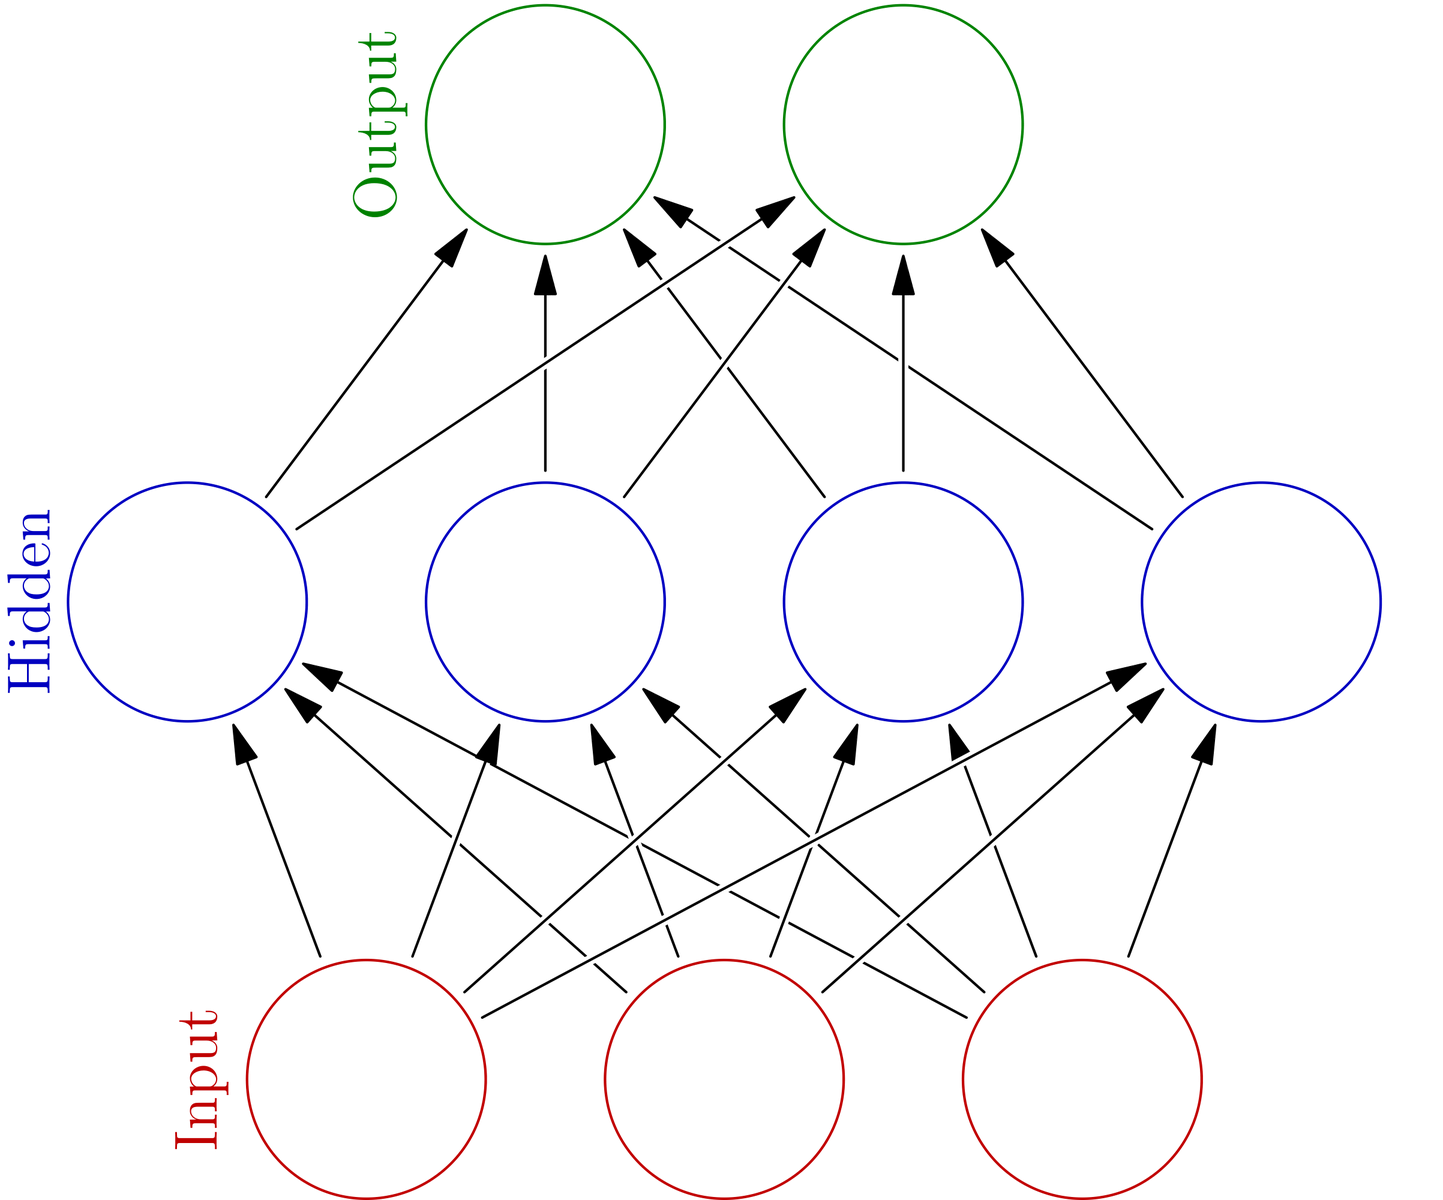
\includegraphics[scale = 0.2]{imm/colored_neural_network-1200x1443.png}
    \label{fig:my_label}
\end{figure}

Quindi fissata una mappa $f$ tra input e output, sulla base degli stimoli $x_k$, la rete cambia i pesi in modo che dopo un numero finito di passi $s$ si abbia l'output $y_k$ tale che $f(x_k)=y_k,\forall\,k>s$ (almeno approssimativamente). Per la modifica bisogna minimizzare un \textbf{criterio di discrepanza} tra risposta della rete e risposta desiderata.\\

%% io non ho aggiunto l'esempio, me lo sono solamente guardato

Viene aumentata la potenza rispetto al percettrone, permettendo una classificazione \textbf{altamente non lineare}.\\ 

\subsubsection{Unità sigmoidi}
Si hanno quindi $u_1,\ldots, u_n$ neuroni divisi in: \begin{itemize} 
    \item unità di input 
    \item unità nascoste 
    \item unità di output 
\end{itemize} 
Si hanno inoltre: 
    \begin{itemize} 
    \item pesi $w_jj$ per ogni coppia che voglio connettere 
    \item stati di attivazione $s_j\in \mathbb{R}$ 
    \item input netto a $u_j$: $n_i=\displaystyle\sum_{i=0}^n w_{ij}\cdot s_i$ \item funzione di transizione sigmoide: $s_j(t+1)=\displaystyle \frac{1}{1+e^{-n_i(t)}}$ 
\end{itemize}

Lo stato di uscita è determinato da una serie di strati profondi. Dato un input $x$, un output target $t$ e un output effettivo $y$. Si consideri la forma quadratica: $E=\frac{1}{2}\sum_j(t_j-y_j)^2$ che dipende anche dagli strati nascosti. 
I pesi vengono modificati usando la seguente formula: $\displaystyle\Delta w_{ij}=-\eta\cdot\frac{\partial E}{\partial w_{ij}}$ poiché: \\ $\displaystyle\frac{\partial E}{\partial w_{ij}}= \frac{\partial E}{\partial n_{j}}\cdot \frac{\partial n_j}{\partial w_{ij}}= \frac{\partial E}{\partial n_{j}}\cdot s_j=(def)-\delta_j\cdot s_j$, dobbiamo determinare  $\displaystyle\delta_j=-\frac{\partial E}{\partial n_{j}}$

Per poter arrivare a determinare quanto ci interessa, dobbiamo utilizzare l'\textbf{algoritmo di retropropagazione}, a sua volta quest'ultimo che si divide in 5 passi.

\subsubsection{Algoritmo di retropropagazione}
I passi da cui è composto sono i seguenti:
\begin{enumerate}
    \item \textbf{Input}: al neurone di input $u_j$ viene assegnato lo stato $x_j$
    \item \textbf{Propagazione}: si calcola lo stato dei neuroni nascosti o di output $u_j$: $s_j=f_j(n_j)$
    \item \textbf{Confronto}: per ogni neurone di output $u_j$, noto l’output atteso $t_j$, si calcola:  $\delta_j=f_j(n_j)\cdot(t_j-y_j))$
    \item \textbf{retropropagazione dell’errore}: per ogni neurone nascosto $u_j$, si calcola: $\displaystyle\delta_j=f_j(n_j)\cdot\left(\sum_h w_{jh}\cdot \delta_h\right)$
    \item \textbf{aggiornamento dei pesi}: si ha: $\displaystyle w_{ij}=w_{ij}+\eta\cdot \delta_i\cdot s_j$
\end{enumerate}
Nelle prime due fasi viene calcolato principalmente l'output, nel terzo verifico l'errore e nelle ultime due aggiorno i pesi.

\begin{algorithm}[H]
    \SetAlgoLined
    \textnormal{Inizializzo ogni} $w_i$ \textnormal{ con un piccolo valore casuale} \\
    \While{\textnormal{Fino al raggiungimento della condizione di terminazione}}{
        \For{\textnormal{ogni input } $\langle x_1, \ldots x_n),t \rangle$}{
            Immetti $(x_1, \dots ,x_n)$ nella rete e calcola l'output $y_k$ \\
            \For{\textnormal{Per ogni unità di output } k}{
                $\delta_k=y_k\cdot(1-y_k)\cdot(t_k-y_k)$ \\        
            }
            \For{\textnormal{Per ogni unità nascosta } h}{
                $\delta_h=y_h\cdot(1-y_h)\cdot\sum_k w_{hk}\delta_k$ \\        
            }
            \For{\textnormal{Per ogni peso } $w_{i,j}$}{
            $w_{ij}=w_{ij}+\Delta w_{ij},\mbox{ con } \Delta w_{ij}=\eta\cdot\delta_j\cdot x_{ij}$
            }
        }
   }
   \caption{Algoritmo di retropropagazione}
\end{algorithm}

Questo algoritmo, che ha una discesa lungo il gradiente rispeto all'intero vettore dei pesi, si generalizza facilmente a grafi orientati arbitrari.\\ Si trova però un \textbf{minimo locale}, non necessariamente \textbf{globale}, e spesso include \textbf{termini di momento} per cambiare la formula dell'aggiornamento dei pesi del tipo: 
$\Delta w_{ij}(n)=\eta\cdot \delta_j\cdot x_{ij}+\alpha\Delta w_{ij}(n-1)$ in modo da avere una sorta di \textit{inerzia} per la variazione dei pesi.\\ 
Ci sono comunque modelli per uscire dai minimi locali.\\ 
Si minimizzano gli errori sugli esempi di training, ma si rischia l'\textbf{overfitting}.\\ 
Tutti questi fattori comportano un addestramento lento ma dopo l'addestramento si ha una rete veloce.\\

L'algoritmo ha diversi limiti:
\begin{itemize}
  \item mancanza di teoremi generali di convergenza
  \item può portare in minimi locali di $E$ 
  \item difficoltà per la scelta dei parametri 
  \item scarsa capacità di generalizzazione 
\end{itemize}
Si possono apportare diverse modifiche per apportare qualche miglioria al modello tramite:
\begin{itemize}
  \item un tasso di apprendimento adattivo: $\eta=g(\nabla E)$
  \item termine di momento $\Delta w_{ij}(n)=\eta\cdot \delta_j\cdot x_{ij}+\alpha\Delta w_{ij}(n-1)$
  \item range degli stati da –1 a 1 
  \item deviazioni dalla discesa più ripida 
  \item variazioni nell'architettura (numero di strati nascosti)
  \item inserimento di connessioni all'indietro
\end{itemize}
% salta le slide a caso
\textit{Le reti \textbf{feedforward} sono state usate in progetti di guida autonoma come \textbf{ALVINN}.}\\
%salta altre slide e non so se bisogna aggiungere altro
